\Chapter{Matematikai modell részletezése}

\Section{Modell specifikálása}

A közlekedésre irányuló modell elkészítéséhez egy olyan modellt kell definiálni, amely elegendő információ leírására képes ahhoz, hogy a közlekedés szimulációja megoldható legyen.
Ezt rengeteg féle képpen meg lehet valósítani, sokféle eleme lehet egy adott térképnek, akár minden egyes előforduló úttípusra, 
szabályra, táblára tekinthetünk úgy, mint a modell egyedi része. Ez a megközelítés viszont lehetségesen túlbonyolítaná a modellt, ezáltal a procedurális generálás
nem adna annyira elfogadható úthálózatot, lehetségesen életszerűtlen helyzetek épülhetnek fel a sok elem megléte, azok elhelyeződése miatt. Sokkal inkább célszerű a 
modell részeként tekinteni a főbb építőelemeket, melyek elegendőek magához az úthálózat generálásához, valamint néhány alapvető szabályt megvalósító elemet, mint például 
a lámpás útkereszteződés, az egyirányú út, valamint a többsávos út.

\Section{A modellben használt elemek}

Matematikailag a modell egy irányított gráfból áll, melynek csomópontjai jelölik az útkereszteződéseket, vagy két egyenes útszakasz között az összekötő részt. Az élek jelölik magát az útszakaszokat, ezeknek az éleknek pedig számos tulajdonságai lehetnek amivel különbséget teszek több elem között. Az élek lehetnek irányítottak is, a modellben ez fogja jelölni az egyes elemeken a haladási útvonalat.

\subsection{Egyenes út}

Alapvető egyenes útszakasz, ennek lehet több paramétere is. Ennek az elemnek elsősorban tartalmaznia kell az úton létező sávok számát.
Az elem leírásához szükség van annak kezdő és végpontjára. További információt ad a modell többi részének, ha tartalmazza egy megközelítőleges égtájnak megfelelő irányt. Ebből következtetni lehet arra, ha például kanyar következik, és ha igen akkor milyen irányban, csak arra van szükség rá hogy megnézzük milyen módon változik az utak hozzávetőleges iránya.

Alapvetően az út olyan szélességű, hogy elfér egymás mellett két jármű, ezért ha több sáv van csak arra kell figyelni, hogy megfelelő helyen közlekedjenek az adott járművek. A gráfon való pozicíójának behatárolásához a kezdő és végpont az ő általa összekötött két csomópontot jelenti.

\subsection{Egyirányú út}

Hasonló az egyenes úthoz, viszont egyértelműen meg kell határozni a két végpont közül melyik a kiindulási, melyik a célpont. Hasonlóan az egyenes szakaszhoz, azzal a különbséggel, hogy ez az út kizárólag 1 sávos.

A gráfot tekintve itt a két összekötött csomópont között egy irányított él lesz, melynek kezdő és végpontjaként egyértelműen el kell jelölni a két pontot.

\subsection{Kanyar}

A kanyar tekinthető tulajdonképpen külön elemnek, de lényegében csak két egymást követő egyenes szakasz, melyek az őket összekötő elem mentén nem egyenes irányban folytatódnak. A kanyar iránya adódik az általa összekötött két egyenes útszakasz irányából.

A gráfon kanyarnak tekinthető az olyan csomópont, melyből csak két él indul ki, ha ez a két él iránya egymástól eltérő, és nem ellentétes.

\subsection{Útkereszteződés}

Három vagy több útszakasz találkozásánál használatos elem. Tulajdonságai közé tartozhat az hogy tartalmaz-e jelzőlámpát az útkereszteződés, vagy sem.
Az útkereszteződés jellemezhető annak középpontjával, valamint az azt érintő utak halmazával.

A gráfon ez azt jelenti, hogy amennyiben egy csomópontból legalább 3 él indul ki, az egy útkereszteződés (\ref{fig:xroad}. ábra).

\begin{figure}[H]
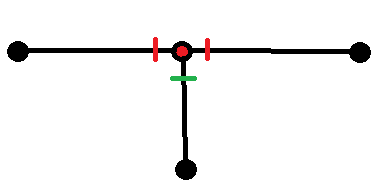
\includegraphics[width=\linewidth]{utkereszt.png}
\caption{Háromágú útkereszteződés lámpákkal}
\label{fig:xroad}
\end{figure}

\subsection{Személygépjármű}

A szimuláció szempontjából a személygépjármű tekinthető az alapvető járműnek. Az autókról nyilván kell tartani azok jelenlegi pozícióját, mely abból adódik hogy éppen melyik élen haladnak, melyik csomópont felé, és attól milyen távolságra vannak. Minden jármű véletlenszerűen kiválasztott útvonalat kap, amin végig kell haladjon. Ezek az útvonalak a teljes gráfon egy-egy részgráfok. A jármű jellemzői közé tartozik annak sebessége, valamint a következő csomópontot elérve a várható haladási iránya, tehát előre, balra, vagy jobbra megy-e tovább. 

Tudnia kell a vele egy úton közlekedő járművekől is, azok pozíciójától függ a viselkedése. A járművek kezdetben véletlenszerű helyen kezdenek, majd ha sikeresen eljutottak a célpontjukhoz 
eltűnnek a modelből (leparkolt kocsinak tekintve). Ezen útvonal kijelölése egy véletlenszerűen kiválasztott csomóponttól indul, ahonnan véletlenszerű irányba indulunk el, majd a következő csomópontot elérve szintén új irányt választunk addig, ameddig vagy zsákutcába nem ér az autó, vagy eléri a paraméterként maximálisan kijelölt úthosszat. Szintén a paraméterezést tekintve ilyenkor új jármű jelenik meg ha jelenleg kevesebb van mint a megadott maximális érték.

\subsection{Autóbusz}

Kissé különlegesebb járműtípus, vonatkozik rá néhány további szabály. Többek között elsőbbsége van megállóból elindulva, valamint ha lehet próbál jobbra tartani,többsávos úton használhatja a külső sávot is egyenes haladásra és balra kanyarodásra. A buszmegállók között megkötött útvonalon kell haladnia, mindegyiknél pedig meg kell állnia. Ha elérte az útvonal végét megfordul, és visszafelé halad végig rajta. A szimuláció teljes ideje alatt az útvonalat követi, kezdetben az útvonal végéről elejétől indul.

Ez az útvonal a gráfot tekintve egy legmélyebb szinten elhelyezkedő véletlenszerűen választott csomópont, valamint a tőle legtávolabb lévő csomópont közötti utat jelenti. Kijelölése könnyen megoldható ezen két csomópont szüleit végigkövetve a középen lévő kiindulási pontig.

\subsection{Buszmegálló}

Autóbusznak elhelyezett megállási pont. Két csomópont közötti él felezőpontján helyezkedik el, ezért leírásához elegendő az adott élt megadni. Szükséges információ a buszmegállók közötti minimum távolság, azaz hány csomópontnak kell lennie legalább két buszmegálló között. Ezt a számot véletlenszerűen fogom meghatározni minden buszmegálló elhelyezése után újra számítva.

Ezen elem egy olyan csomópont, amelyből nem indul él, és nem is tart belé él.

\subsection{Épületek}

A gráf létrejötte után kijelölendő elemek. Az élek két oldalán helyezkednek el a házak, amelyek az alacsonyabb szinten lévő csomópontok között blokkházak, magasabb szinteknél pedig kertesházak. Az út két oldalán lévő elhelyezkedés szimmetrikus. A blokkok magassága változó (\ref{fig:builds}. ábra).

\begin{figure}[H]
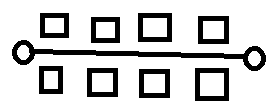
\includegraphics[width=\linewidth]{epulet.png}
\caption{Út két oldalán lévő épületek}
\label{fig:builds}
\end{figure}

\subsection{Park}

Szintén a gráf létrejötte után kerül elhelyezésre, kizárólag az utakkal teljesen közbezárt területeken. Az adott területen belülre fák kerülnek, valamint egy szökőkút (\ref{fig:parkmodel}. ábra).

\begin{figure}[H]
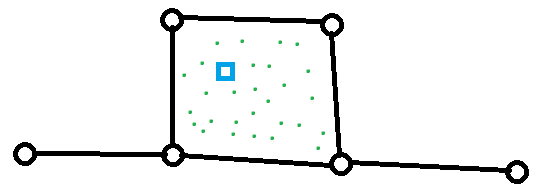
\includegraphics[width=\linewidth]{park.png}
\caption{Elkerített részen lévő park, kék négyzettel jelölve a szökőkutat, zöld pontokkal a fákat}
\label{fig:parkmodel}
\end{figure}

\subsection{Útvonal}

Ez az egy járműhőz tartozó egyedi haladási vonala az úthálózaton. Nem ugyan az, mint az útvonal éleinek kezdő és végpontja, ugyanis itt egyértelműen ki kell jelölni annak a sávnak a pontjait, amelyikben a jármű haladni fog. Útkereszteződésben ez segít a helyes irányba való kanyarodásban (\ref{fig:path}. ábra).

\begin{figure}[H]
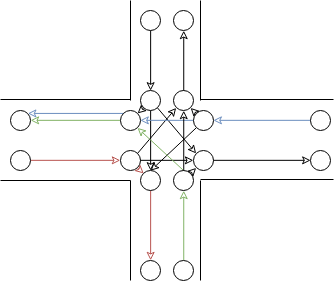
\includegraphics[width=\linewidth]{ut.png}
\caption{Egy útkereszteződésbeli útvonalakat kijelölő pontok. Példa útvonal balra kanyarodáshoz (zöld), jobbra kanyarodáshoz (piros), egyenes haladáshoz (kék).}
\label{fig:path}
\end{figure}

\subsection{Közlekedési szabályok}

Az alapvető közlekedési szabályok többsége, amelyet a járműveknek követniük kell, általában attól az elemtől függ ahol haladnak, valamint attól amelyhez tartanak. Ilyenek az alábbiak.
\begin{itemize}
\item Egyirányú útra csakis a kijelölt útirányban hajthatnak rá a járművek.
\item Ha az út több sávot tartalmaz, a külső sáv csak jobbra kanyarodásra alkalmas, a belső sáv balra kanyarodásra, illetve egyenes haladásra
\item Ha az útmenti buszmegállóból elindulni készül a busz, a többi járműnek elsőbbséget kell neki adnia.
\item Jelzőlámpával ellátott útkereszteződésbe nem hajthat be ha a lámpa piros, ha aközben vált hogy benne van akkor még áthaladhat.
\end{itemize}

\Section{A modell kritériumai}

\subsection{Generálási szempont}

Magának az úthálózatnak a generálására vonatkozóan a következők a célok.
\begin{itemize}
\item Viszonylag kevés elemből álljon össze a generált úthálózat.
\item Ne legyen életszerűtlen az összeállított úthálózat.
\item Tartalmazza az alapvető közlekedési helyzetek szimulálására szükséges elemeket.
\item Vizuálisan emlékeztessen egy átlagos városra.
\item Bizonyos mértékig paraméterezhető legyen, főleg a méreteket érintve.
\end{itemize}

\subsubsection{Elemek száma}

Az említett viszonylag kevés (pontosabban kevés különbözű típusú) elem azért szükséges, hogy ne legyenek túl specifikusak a modell nagyobb részei, hanem akár könnyedén egyik elem bővítésével elő lehessen állítani egy másikat. Ilyen például a modellben az egyenes szakasz, melyből kis változtatással előáll az egyirányú út.

\subsubsection{Életszerű úthálózat}

Röviden annyit tesz, hogy nem tartalmaz olyan területeket ahol össze van szűkítve kis területen rengeteg út. Tehát legyen minimális hely kihagyva az utak között az épületeknek. Életszerűtlennek tekinthető továbbá az is, ha egy útkereszteződésből rengeteg út indul ki, azaz 5-6 avagy annál több. Ezért a modellben az útkereszteződés maximálisan 4 utat köthet össze.

\subsubsection{Közlekedési helyzetek}

Legyen benne jelzőlámpával ellátott útkereszteződés, többsávos út, egyirányú út, valamint buszmegálló. Ezek az elemek szükségesek minden esetben, hogy a szimuláción meg lehessen jeleníteni a lámpák működését, a többsávos utak eseten a járművek sávválasztását és tartását, egyirányú út irányának a betartását, és buszmegállónál a busz megállását, neki járó elsőbbség megadását.

\subsubsection{Átlagos város képe}

Egy várost átlagosnak (tipikusnak) tekintünk akkor, ha a központtól kifelé haladva ritkul az úthálózat, valamint a többsávos utak az előreláthatólag forgalmasabb helyeken vannak elhelyezve. Ennek érdekében a modellben elhelyezett csomópontok átlagosan kevesebb élt indítanak magukból, minél távolabb vannak a gráf kiindulási pontjától, azaz a középponttól.

\subsubsection{Paraméterezés}

Ki lehessen jelölni, hogy a generálás meddig tartson, azaz hány csomópontot terjesszen ki. 

\subsection{Szimulációs szempont}

A már legenerált úthálózaton a szimulációra tekintve az alábbi elvárások vonatkoznak.
\begin{itemize}
\item A járművek kövessék a modellben definiált alapvető szabályokat.
\item A szimuláció bizonyos mértékben paraméterezhető legyen, főleg a járművek számát illetően.
\item Reagáljanak egymásra a járművek
\item Ne legyen életszerűtlen a járművek viselkedése.
\item Teljesítmény szempontjából elfogadható legyen egy adott méretig.
\end{itemize}

\subsubsection{Szabályok}

A már előbbiekben leírt szabályoknak megfelelően közlekedjenek a járművek, haladási útjukat azok alapján válasszák meg.

\subsubsection{Paraméterezés}

Meg lehessen adni mennyi jármű legyen maximálisan egyidőben az úthálózaton, külön értve a buszokat ettől. Továbbá az is megadható legyen milyen gyakorisággal jelenik meg személygépjármű, és mekkora lehessen a neki kijelölt útvonal maximális hossza csomópontokban mérve.

\subsubsection{Reagálás}

Ha egy jármű közelít egy másik felé kezdjen lassítani. Ez a lassítás függjön a távolság mértékétől, ha elég közel kerül hozzá teljesen álljon meg. Csak akkor induljon el egy jármű, ha haladási útját nem állja el másik jármű. Közúti baleset, azaz ütközés esetén a két érintett jármű kis idő után tűnjön el, ezzel szemléltetve az elszámolás, elvontatás folyamatát.

\subsubsection{Életszerű viselkedés}

A járművek tartsák az út vonalát, ne térjenek át a szembe sávba. Gyorsítás és lassítás viszonylag realisztikusan történjen, ne pedig hirtelen. Kanyarodás előtt igyekezzenek lelassítani, kanyart pedig végig lassan bevenni.

\subsubsection{Teljesítmény}

A szimuláció mérete alatt mind az úthálózat csomópontjainak, mind az egyszerre megjelenő autók számát értem. Abban az esetben, ha ezek az értékek nem kimagaslóan nagyok, a szimulációnak lényegesebb teljesítményromlás nélkül kell futnia.
